\newpage
\NewsItem{Luftfeuchtigkeitsmessung mittels Tauspiegelverfahren}
\begin{multicols}{3}
%%======================================================================== Text Einfügen
{ \centering
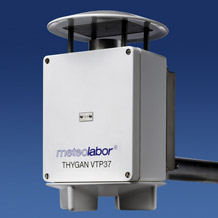
\includegraphics[width=\columnwidth]{graphics/thygan.jpg}
\captionof{figure}{Thygan \cite{MeteolaborkeineAngaben}}
\label{thygan}
}
\vfill\columnbreak
Dieses Verfahren beruht auf der physikalischen Beziehung zwischen Wasserdampfgehalt und Kondensationstemperatur des Wasserdampfes in einem Gasgemisch. Ein Spiegel wird abgekühlt bis mit einem optischen Element Kondensat detektiert wird. Das optische Element registriert die Reflexionsverhältnisse des Spiegels, womit dieser auf die Taupunkttemperatur eingeregelt wird. Die Taupunkttemperatur ist erreicht wenn die Temperatur des Spiegels diese unterschreitet und dadurch beschlägt, womit die Reflexion beeinträchtigt wird. Die Temperatur des Spiegels wird mit einem Temperaturfühler gemessen, dazu muss dieser sich direkt am Spiegel befinden. Mit dieser Taupunkttemperatur wird dann über eine Kennlinie der Wert der Luftfeuchtigkeit berechnet. \cite{Hesse2014}\cite{MeteoSchweiz2014}\\[0.5cm]
Der Thygan hat einen Messbereich der Lufttemperatur von -50$^{o}$C bis 50$^{o}$C und eine Taupunktstemperatur von -65$^{o}$C bis 50$^{o}$C. Die Auflösung der Temperaturwerte sind 0.1K, sowie auch 0.1\% der relativen Luftfeuchte. Die Messgenauigkeit ist Temperaturabhängig und beträgt $\pm$0.15K von -20$^{o}$C bis 50$^{o}$C und $\pm$0.25K von -65$^{o}$C bis -20$^{o}$C. \cite{Meteolabor2018}

\end{multicols} 
